\documentclass[a4paper,10pt,twoside]{article}

%\usepackage{ucs}
\usepackage[utf8]{inputenc}
%\usepackage{babel}
%\usepackage{fontenc}
\usepackage[pdftex]{graphicx}

\usepackage[pdftex]{hyperref}

\author{Jessamy Mol}
\title{Tutorial 2a exercise paper}
\date{09/14/17}

\begin{document}

\maketitle

\begin{center}
 \texttt{jessamy.mol@gmail.com}
\end{center}

\section{Introduction}
\label{sec:intro}

Wow cool introduction! Everyone will understand section \ref{sec:sum} now.

\section{Summary}
\label{sec:sum}

\begin{figure}[h]
 \begin{center}
  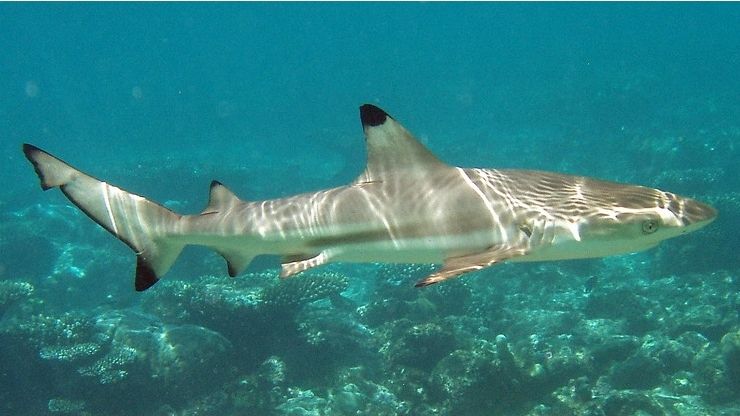
\includegraphics[width=5cm]{shark.jpg}
  \caption{A beautiful black tip reef shark.}
  \label{fig:shark}
 \end{center}
\end{figure}

Figure \ref{fig:shark} shows the beauty of a \textit{black tip reef shark}~\footnote{All sharks are beautiful}. Image was taken from the interwebs~\cite{webs}.  

\subsection{More sharks}
\label{sec:more}

\begin{table}[h]
 \begin{center}
  \caption{Some different sharks}
  \begin{tabular}{c|c}
   \textbf{Type} & \textbf{Awesomeness (on a scale from 1 to 10)} \\ \hline 
   Black tip reef shark & 10 \\
   Hammerhead & 10 \\
   Great white & 10 \\
   Nurse shark & 10 \\
  \end{tabular}

 \end{center}
\end{table}

\section{Maths}
\label{sec:maths}

\begin{equation}
\label{eq:random}
 \omega = \left(\frac{2x^4}{\hbar}\right)^2
\end{equation}

We now know that:
\begin{itemize}
 \item All sharks are:
 \begin{enumerate}
  \item Awesome 
  \item Beautiful
  \item Cool
 \end{enumerate}
 \item Everyone should love sharks
\end{itemize}

\begin{verbatim}
 \usepackage{verbatim}
 Some code 
 print 10**5 
\end{verbatim}




\begin{thebibliography}{99}
 \bibitem{webs} The interwebs source \url{https://en.wikipedia.org/wiki/Blacktip_reef_shark}
\end{thebibliography}


\end{document}
